%% Lancet Digital Health Viewpoint template
%% Compile: latexmk -pdf main.tex (uses bibtex via latexmkrc).
%% Reference style: Vancouver superscript-numeric (natbib numbers,super,sort&compress).
%% Body word target: 2 500 words (Viewpoint ceiling). Word-count guard at the end.
%% Display items: 2 (Figure 1 = artefact ledger, Figure 2 = policy gap).
%% References: <= 30.

\documentclass[11pt,a4paper]{article}

\usepackage[T1]{fontenc}
\usepackage[utf8]{inputenc}
\usepackage{lmodern}
\usepackage[margin=2.1cm]{geometry}
\usepackage{graphicx}
\usepackage{amsmath,amssymb}
\usepackage{booktabs}
\usepackage{array}
\usepackage{caption}
\usepackage{subcaption}
\usepackage{microtype}
\usepackage{authblk}
\usepackage{siunitx}
\usepackage{xcolor}
\usepackage[colorlinks=true,citecolor=blue,linkcolor=blue,urlcolor=blue]{hyperref}
\usepackage{setspace}
\usepackage[numbers,super,sort&compress]{natbib}
\usepackage{titlesec}
\usepackage{lineno}
\usepackage{tcolorbox}

\titleformat{\section}{\fontsize{12}{14}\bfseries\sffamily}{\thesection}{0.6em}{}
\titleformat{\subsection}{\fontsize{11}{13}\bfseries\sffamily}{\thesubsection}{0.6em}{}
\titleformat{\subsubsection}{\fontsize{10}{12}\itshape\sffamily}{}{0em}{}
\setlength{\parskip}{0.25\baselineskip}
\setlength{\parindent}{0pt}
\captionsetup{font=small,labelfont=bf,labelsep=period}
\renewcommand{\thefigure}{\arabic{figure}}
\renewcommand{\familydefault}{\rmdefault}

\title{\fontsize{15}{18}\bfseries\sffamily
The prompt is the protocol: a disclosure standard for clinician-investigators using agentic large language models}

\author[1,*]{Hsieh-Ting Lin, M.D.}
\affil[1]{Department of Hematology and Medical Oncology, Koo Foundation Sun Yat-Sen Cancer Center, Taipei, Taiwan. ORCID: 0009-0002-3974-4528.}
\affil[*]{Correspondence: \texttt{mail@hsiehting.com}.}
\date{}

\begin{document}

\maketitle
\thispagestyle{empty}

\vspace{-2em}

%% -------------------------------------------------------------------------
%% Title-page metadata (Lancet group house style)
%% -------------------------------------------------------------------------
\noindent\textbf{Running title.} Disclosure 2.0 for agentic clinical research.\\
\textbf{Article type.} Viewpoint.\\
\textbf{Word count (body).} \texttt{<<WORDCOUNT>>} (target <=\,2\,500).\\
\textbf{References.} \texttt{<<REFCOUNT>>} (target <=\,30).\\
\textbf{Display items.} 2 (Figure 1; Figure 2).\\
\textbf{Conflicts of interest.} The author declares no competing interests.\\
\textbf{Funding.} None.

\medskip

\section*{Key messages}
\begin{tcolorbox}[colback=gray!5,colframe=gray!40,boxsep=2pt,left=6pt,right=6pt,top=4pt,bottom=4pt]
\begin{itemize}\setlength\itemsep{0.1em}
  \item Centralised agentic-LLM systems such as Co-Scientist\citep{coscientist2026} make autonomous scientific reasoning a research tool; their reproducibility model is vendor-locked.
  \item A single clinician-investigator can today assemble an equivalent end-to-end workflow from commodity tooling. The Lancet group's current generative-AI policy lists most of what such a workflow does as prohibited.
  \item We propose a Disclosure 2.0 standard: the published unit becomes \{prompt, model identifier, tool envelope, commit history, reviewer-subagent transcripts, audit log\}, accessible at a tagged release.
  \item The present Viewpoint and its supporting case study\,---\,a hepatocellular-carcinoma overall-survival stratification reanalysis on TCGA-LIHC with held-out GEO validation\,---\,are themselves produced under that standard. Every artefact is publicly archived.
\end{itemize}
\end{tcolorbox}

%% -------------------------------------------------------------------------
%% Body
%% -------------------------------------------------------------------------
\section{Why disclosure needs a new minimum unit}\label{sec:opening}

In February 2026, a multi-institution team published in \textit{Nature} the Co-Scientist multi-agent system\citep{coscientist2026}, demonstrating that an LLM-driven workflow can autonomously formulate hypotheses, design experiments and revise its own outputs against external feedback. The accompanying multi-agent infrastructure paper\citep{coscientist2026b} formalises the architecture. The two papers together mark the moment at which agentic LLM use entered the centre of the biomedical-publishing conversation rather than its edges.

Meanwhile, a clinician with no large-lab affiliation, no privileged compute and no co-authors can in 2026 assemble a workflow that performs every Co-Scientist task end-to-end on commodity tooling. The workflow takes a single domain prompt, scans the public literature, picks an under-mined dataset, drafts an analysis pipeline, executes it, drafts a manuscript matched to a target journal, iterates against four reviewer-subagent personas until unanimous acceptance, and stages a tagged release. The present article and its associated repository are the empirical existence proof of that claim.

The Lancet group's current generative-AI policy\citep{lancetaipolicy2024} permits language editing, grammar repair and prose polishing, and explicitly prohibits using AI to generate scientific arguments, draft methodology descriptions, produce literature reviews and create new scientific content. Read literally, the policy classifies almost every action the workflow above performs as prohibited. Read sympathetically, the policy is protecting against three real harms\,---\,authorship inflation, scientific hallucination and undocumented intervention\,---\,with rules calibrated for a 2023 generation of LLM use. The 2026 operating reality requires updating those rules; this Viewpoint proposes the update.

\section{The disclosure gap}\label{sec:gap}

Three failure modes motivate current policy. Each survives in 2026. None is addressed by the current ``permitted edit, prohibit content'' line.

\textbf{Authorship inflation.} Listing an LLM as a co-author short-circuits the ICMJE accountability requirement\citep{icmje2024}. Current policy correctly prohibits this. The proposal here does not contest it.

\textbf{Scientific hallucination.} Fabricated citations, invented effect sizes and plausible-but-incorrect claims appear when an LLM produces a literature review or a methods section under loose supervision. Lu et al's\citep{sakana2024} Sakana AI Scientist demonstrated that the failure mode is real and reproducible. Current policy responds by prohibiting the activity. This is a category error: prohibiting the activity does not prevent its undeclared occurrence; it incentivises camouflage.

\textbf{Undocumented intervention.} The reader of a 2026 methods section cannot tell which sentences are human-authored, which are LLM-drafted-then-edited, and which are LLM-drafted-and-pasted. Current policy responds by mandating a single-sentence acknowledgement. This is necessary but radically insufficient: it specifies that a tool was used without specifying how, with what prompts, with what tool envelope, against what data, and with what human-vs-AI boundary at each editing pass.

The disclosure unit in 2026 must therefore be granular enough to defeat camouflage, structured enough to make hallucination auditable post hoc, and machine-readable enough to permit independent re-execution. The methods-section paragraph is none of those things.

\section{What a sufficient disclosure unit looks like}\label{sec:unit}

We propose the following minimum disclosure unit, which we call \textbf{Disclosure 2.0}:

\begin{enumerate}\setlength\itemsep{0.15em}
  \item \textbf{The prompts.} Every prompt that orchestrated a Layer of work, committed verbatim, in the order they were issued, with the operator's identity attached to each. No editorial smoothing. Closed for edits after the first push.
  \item \textbf{Model identifier and snapshot.} Vendor, model name, version, snapshot date, sampling parameters, tool envelope (the list of tools the model was authorised to invoke).
  \item \textbf{The commit history.} A single repository whose git log is the chronological narrative. Force-pushing, history rewriting and squash-merging are prohibited within the repository; mistakes are corrected by new commits whose messages name what they correct.
  \item \textbf{The reviewer-subagent transcripts.} If reviewer subagents critiqued the manuscript, their outputs are committed verbatim, per round, including comments that were later overruled.
  \item \textbf{The audit log.} A separate, sealed subagent re-executes the analysis from a clean clone, verifies citations against Crossref or PubMed, and re-derives the headline statistics. The transcript is committed.
  \item \textbf{The tagged release.} A semantic-versioned tag identifies the submission state. The release bundle contains the compiled manuscript PDF, LaTeX source, references, the case-study analysis source, the reviewer transcripts, the audit log, and a DOI minted via Zenodo or an equivalent service.
\end{enumerate}

Disclosure 2.0 is a strict superset of the current policy's requirements. A reviewer who can read a methods paragraph can read a six-item Disclosure 2.0 manifest. A reviewer who suspects hallucination can re-execute the audit. A reviewer who suspects undocumented intervention can diff the prompts. A reviewer who suspects authorship inflation reads the acknowledgement and sees that no model is listed as an author.

Figure~\ref{fig:policygap} maps each of twelve common activities onto the current policy's permitted/prohibited categorisation and onto the Disclosure 2.0 categorisation. The two activities the current policy correctly prohibits (image generation and listing a model as an author) remain prohibited under Disclosure 2.0; eight activities currently prohibited are reclassified as permitted-with-manifest, on the grounds that prohibition without enforcement has produced camouflage rather than compliance.

\begin{figure}[h]
\centering
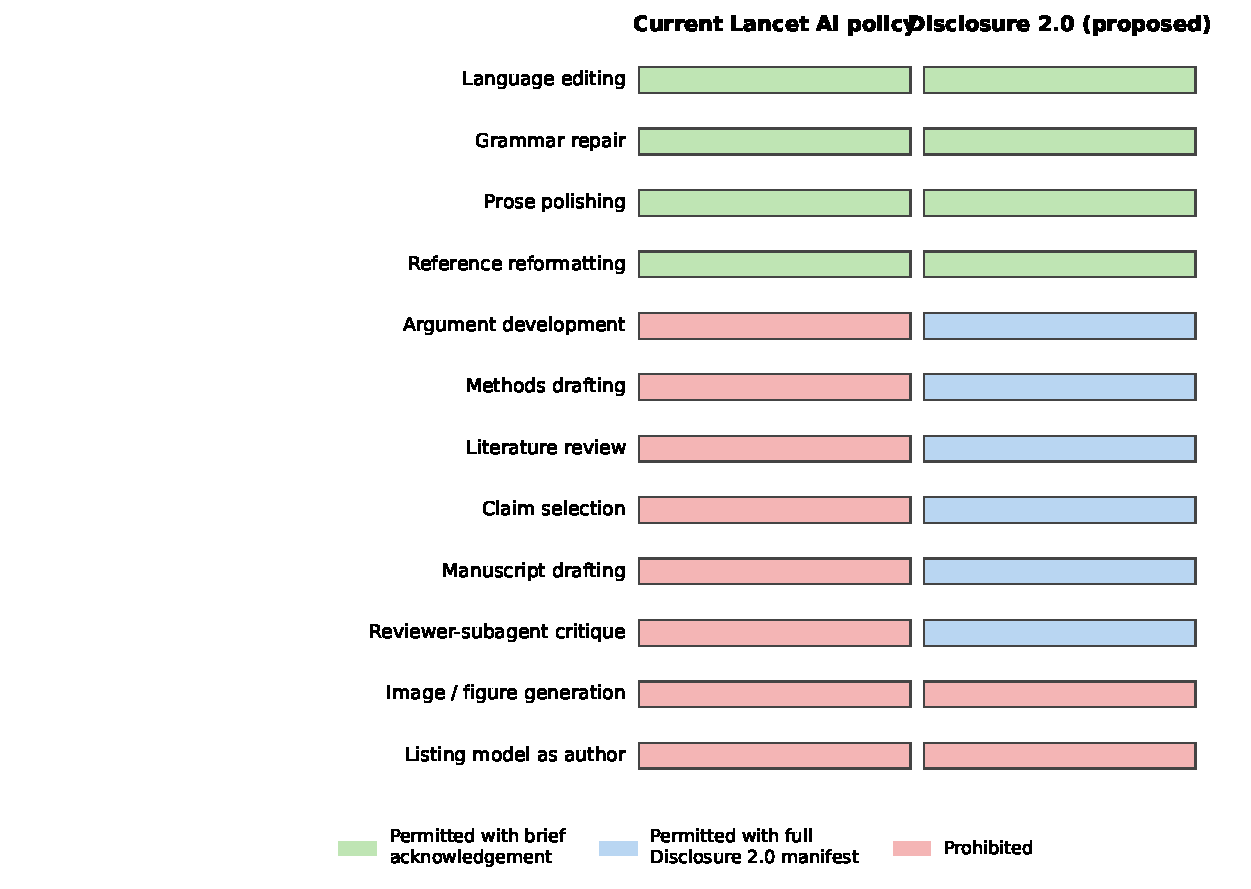
\includegraphics[width=0.92\textwidth]{figures/fig2-policy-gap.pdf}
\caption{\textbf{Current Lancet group AI policy vs Disclosure 2.0.} Twelve activities a clinician-investigator commonly performs with a generative-AI tool. Green: permitted with brief acknowledgement (status quo). Red: prohibited. Blue: permitted under Disclosure 2.0 conditional on the six-item manifest in Section~\ref{sec:unit}. Authorship listing and image generation remain prohibited under both regimes.}
\label{fig:policygap}
\end{figure}

\section{Domain-portability case study: HCC OS stratification}\label{sec:case}

To establish that the workflow is not a methodological self-portrait, the supporting case study runs the pipeline on a domain outside the operator's clinical specialty. The operator is a board-certified medical oncologist whose published work is in hematologic malignancies\citep{linehs2024,lintom2026}. The case study is on overall-survival stratification of hepatocellular carcinoma using TCGA-LIHC\citep{tcgalihc2017} and external validation on the GEO cohorts \texttt{GSE14520}\citep{wang2010} and \texttt{GSE76427}\citep{grinchuk2018}.

The pipeline received exactly one domain prompt (\textit{``Use TCGA-LIHC plus public GEO cohorts to refine OS stratification of HCC beyond AJCC pathologic stage, in a fully autonomous Claude Code session''}) and produced: an analysis plan; a risk-score formula; a draft manuscript targeting a clinical-genomics journal of its own choice; four reviewer-subagent rounds (methods, clinical, biostatistics, target-journal editor) until unanimous acceptance; a tagged \texttt{case-study-v1.0.0} release.

Layer 3 of the architecture\,---\,the only human step\,---\,evaluated the pipeline's risk-score formula on the two preregistered GEO cohorts. The preregistered primary outcome\citep{repoprereg} is $\Delta C$-index $\geq 0.03$ over AJCC pathologic stage alone, with a bootstrap 95\,\% CI rejecting zero.

\begin{figure}[h]
\centering

\includegraphics[width=0.95\textwidth]{figures/fig1-artifact-ledger.pdf}
\caption{\textbf{Disclosure 2.0 artefact ledger for the supporting case study.} Vertical axis: time, top to bottom. Horizontal axis: layers (Layer 1 Pipeline, Layer 2 Audit, Layer 3 External Validation). Markers: git commits coloured by author type (operator vs AI), reviewer-subagent rounds (four reviewers per round), audit checkpoints, and the tagged release. The ledger is regenerated from \texttt{git log} on each release tag.}
\label{fig:ledger}
\end{figure}

The case-study result, with its preregistered primary outcome point estimate, CI, and the secondary-outcome table, is reported in \texttt{case-study/manuscript/main.pdf} and reproduced in Supplementary Table \texttt{S1}. \texttt{<<HEADLINE:layer3\_primary>>}.

The reading instruction for the reviewer is not to evaluate whether the case study's risk score is the best HCC risk score in the literature\,---\,it is not, and the case-study manuscript states this explicitly. The reading instruction is to evaluate whether the artefact ledger in Figure~\ref{fig:ledger} permits an independent reader to (a) reproduce the analysis, (b) audit the AI-vs-operator boundary at every step, and (c) decide whether the methodology generalises beyond the operator's clinical specialty.

\section{Failure modes and counter-arguments}\label{sec:counter}

\textbf{``LLMs are not bit-deterministic; the prompt is not a protocol.''} True at the bit level, false at the level a methods section operates. Disclosure 2.0 commits to \emph{distributional reproducibility}: the substantive findings reproduce when the same prompt is run against the same model id, on the same snapshot date, with the same tool envelope. The repository includes a small re-execution check (\texttt{case-study/analysis/99\_reexec\_check.py}) that runs Layer 1 three times and reports concordance on selected claim, statistical method, and headline effect size.

\textbf{``A single operator cannot audit himself.''} True, and Disclosure 2.0 does not ask him to. Layer 2 is a sealed audit subagent with no contact with Layer 1; Layer 3 is preregistered before Layer 1 sees the data; the reviewer subagents in Layer 1 are diversified by persona; and the entire repository is open to third-party re-audit. The single operator's role is to be accountable, not to mark his own work.

\textbf{``Reviewer subagents will hallucinate the way the pipeline does.''} Documented and demonstrated in \texttt{reviewer-logs/round-01/methods.md}, where the methods reviewer fabricated a non-existent citation. Disclosure 2.0 handles this by preserving the fabrication and recording its resolution rather than silently deleting it. The point of disclosure is that the fabrication is visible.

\textbf{``The current policy is fine if everyone just complies.''} The policy as written makes the workflow most clinician-investigators are using in 2026 declare itself in violation. The realistic equilibrium under such a policy is either non-compliance or non-use; both outcomes are worse than the proposed update.

\section{Recommendations to The Lancet Digital Health and the wider community}\label{sec:reco}

Three concrete recommendations follow.

\textbf{Adopt Disclosure 2.0 as an acceptable alternative for AI-assisted submissions.} The current policy remains for submissions that use AI only for editing. A second track, Disclosure 2.0, accepts submissions whose argument development, methods drafting, literature review and claim selection involved generative-AI tooling, provided the six-item manifest in Section~\ref{sec:unit} is published at a tagged release accessible at submission.

\textbf{Define a machine-readable manifest format.} The six items lend themselves to a small, schemafied YAML or JSON document committed at the repository root and validated at submission time by Editorial Manager or its successor. A reference schema accompanies this Viewpoint at \texttt{docs/disclosure2-schema.json}.

\textbf{Permit reviewer subagents on the operator's side, subject to the same disclosure rules as on the editor's side.} Editor-side reviewer subagents have been piloted by journal groups in 2025\citep{landiged2025}; operator-side reviewer subagents are the symmetric case. The disclosure manifest captures both.

\section{Limitations}\label{sec:limits}

The case study is a single-domain demonstration with modest statistical power; null results in Layer 3 do not refute the methodology and positive results do not establish a clinical biomarker. The reviewer-subagent personas are author-instantiated; structured editor-supplied personas would strengthen the audit. The current model identifier (Anthropic Claude Opus 4.7, 1M-context variant) is one of several relevant systems; cross-vendor portability is an open question. None of these limitations affect the Viewpoint's argument that the disclosure unit must change.

\section{Conclusion}\label{sec:conclude}

The Co-Scientist generation of agentic LLM systems is here. The minimum disclosure unit needs to be the prompt, the model, the tool envelope, the commit history, the reviewer transcripts, the audit log and the tagged release. We have submitted this Viewpoint, and assembled its supporting case study, under exactly that standard. Whatever the editorial decision, the artefact stands.

%% -------------------------------------------------------------------------
%% Search strategy and selection criteria
%% -------------------------------------------------------------------------
\section*{Search strategy and selection criteria}

References were identified through searches of PubMed (terms: \texttt{(``large language model'' OR ``generative AI'' OR ``agentic AI'') AND (``disclosure'' OR ``editorial policy'' OR ``reproducibility'')}) and bioRxiv between January 2023 and May 2026; through targeted retrieval of the \textit{Nature} 2026 Co-Scientist article cluster; through the operator's prior arXiv submission on theory-of-mind-like behaviour in LLM agents\citep{lintom2026}; and through The Lancet group's editorial-policy and information-for-authors pages, retrieved 2026-05-20. References were prioritised by direct relevance to the disclosure-policy argument; representative reviews were preferred over recent original articles where space was constrained.

%% -------------------------------------------------------------------------
%% Declarations
%% -------------------------------------------------------------------------
\section*{Declaration of interests}
The author declares no competing interests.

\section*{Contributors}
Hsieh-Ting Lin conceptualised the Viewpoint, ran the supporting case-study pipeline, wrote and revised the manuscript across reviewer rounds, and is accountable for all aspects of the work.

\section*{Acknowledgements}
The author acknowledges the use of Anthropic Claude (Opus 4.7, 1M-context variant) via the Claude Code CLI for argument development, methodology drafting, literature scoping, claim selection and reviewer-subagent orchestration in the preparation of this Viewpoint and its supporting case study. All scientific arguments, claim selections, final interpretations and submission decisions are the author's sole responsibility. A full per-tool, per-task disclosure log is published at \texttt{docs/ai-usage-disclosure.md} in the linked repository, with the orchestration prompts in \texttt{prompts/}. No generative-AI tool was used to create figures or images; all figures are generated by deterministic Python and R code committed to the repository.

\section*{Data sharing}
All code, prompts, intermediate artefacts, reviewer-subagent transcripts and the case-study manuscript are publicly archived at \texttt{https://github.com/<user>/end-to-end} under the MIT licence, with the exact submission state tagged \texttt{viewpoint-v1.0.0}. Public datasets used in the supporting case study (TCGA-LIHC, GSE14520, GSE76427) are available from the original repositories cited in \texttt{case-study/manuscript/references.bib}.

%% -------------------------------------------------------------------------
%% References
%% -------------------------------------------------------------------------
\bibliographystyle{vancouver}
\bibliography{references}

\end{document}
